\documentclass[a4paper,11pt]{article} %Selecionando a classe que gera artigos.

%PACOTES ABNT
\usepackage[brazil]{babel} % Pacote para usar portugues.
%Babel traduz como “table of contents“, “chapter” e “section“, sejam impressas como “sumário”, “capítulo” e “seção”, respectivamente.

\usepackage[T1]{fontenc} %Pacote para copiar palavras com acentuação do pdf de um documento feito em LaTeX que tenha usado esses pacotes resultará nas palavras corretamente acentuadas

\usepackage[utf8]{inputenc} % Pacote para poder usar acentuação no arquivo .tex

%\usepackage{biblatex}


\usepackage{graphicx} %Pacote para inserir Figuras.

\usepackage[top=2.0cm,right=2.0cm,left=2.0cm,bottom=2.0cm]{geometry} %Pacote de Margens

\usepackage{enumerate} %Pacote para usar marcadores.

\usepackage[onehalfspacing]{setspace} %Pacote espaçamento 1,5 cm.

\usepackage[alf]{abntex2cite} % configura o sistema  de citações e referências para o estilo ABNT.


% alf = estilo autor-data, para citações.

%Para mais estilos de citações visite https://www.overleaf.com/learn/latex/Biblatex_bibliography_styles

%PACOTES ESSENCIAIS
\usepackage{graphicx,xcolor,comment,enumerate,multirow,multicol,indentfirst} %Pacote para inserir figuras, tabelas, editar cores das tabelas, numeração "Automática das figuras e tabelas", identar tabelas e figuras.


%PACOTES DE MATEMÁTICA
\usepackage{amsmath,amsthm,amsfonts,amssymb,dsfont,mathtools,blindtext} %Pacotes básicos de matemática.

\usepackage{sectsty}% http://ctan.org/pkg/sectsty
\usepackage{titlecaps}% http://ctan.org/pkg/titlecaps
\sectionfont{\normalsize\MakeUppercase}


\usepackage{fancyhdr}  % Para adicionar o rodapé
 %Pacotes principais

\fancypagestyle{empty}{%
\fancyhf{}% clear all header and footer fields
\fancyfoot[L]{Linguagem e Descrição de Hardware} % except the center
\fancyfoot[R]{\thepage} % except the center
% \fancyfoot[R]{ISSN: 2178-9959} % except the center
\renewcommand{\headrulewidth}{0pt}%
\renewcommand{\footrulewidth}{0pt}%
}
\pagestyle{empty}

\begin{document} %Begin Inicia o Documento

%--------------------------------     NÃO ALTERAR    ----------------------------------------%
\begin{center}

% \begin{table}[!h]
% \centering
% \resizebox{\textwidth}{!}{
% \begin{tabular}{lr}
% %\multirow{4}{*}{
\includegraphics[width=80px]{logo_reitoria.png}} &
% % \multirow{6}{*}{
\includegraphics[width=120px]{logo_conict.png}}                                                                     & 
% % \multirow{6}{*}{
\includegraphics[width=190px]{logo_reitoria.png}} \\
% \multirow{1}{*}{
%   \centering
%   % 
\includegraphics[width=120px]{logo_conict.png}
%   } &
% \multirow{6}{*}{
%   \centering
%   
\includegraphics[width=130px]{logo_ifsp.png}
%   } \\
%                         &                                                        %                    &            
%                         \\
%                         &                                                         %                                    &                         
%                         \\
%                         & \multicolumn{1}{l}{\textbf{}}                          %                                     &                        
%                         \\
%                         & \multicolumn{1}{l}{\textbf{}}                          %                                     &                        
%                         \\
%                         %& 
%                         \multicolumn{2}{c}{\large{\textbf{Linguagem e Descrição de Hardware}}} \\
%                         %& \multicolumn{1}{l}{}   
% \end{tabular}
% }

% \end{table}

\begin{table}[!h]
  \centering
  \resizebox{\textwidth}{!}{
  \begin{tabular}{c}
  
\includegraphics[width=130px]{logo_ifsp.png} \\
  \large{\textbf{Linguagem e Descrição de Hardware}} \\
  \end{tabular}
  }
\end{table}

%-------------------------------------------------------------------------------------------------%



%%%%%%%%%%%%%%%%%%%%%%%%%%%%%  ALTERAR TÍTULO, AUTORES  %%%%%%%%%%%%%%%%%%%%%%%%%%%%%%%%%%%%%%%%%%%%%

\textbf{Greatest Common Divisor - (GCD)}\vspace{0.5cm}

Giovanna Fantacini$^1$, 
Higor Grigorio$^2$, 
Leonardo Reneres$^3$, 
Luis$^4$, 
Raul Prado Dantas$^5$


%%%%%%%%%%%%%%%%%%%%%%%%%%%%%%%%%%%%%%%%%%%%%%%%%%%%%%%%%%%%%%%%%%%%%%%%%%%%%%%%%%%%%%%%%%%%%%%%%%%%%





%----------------------------------APAGAR TABELA COMEÇO--------------------------------------------%

% \begin{table}[!h]
% \centering
% \resizebox{\textwidth}{!}{%
% \begin{tabular}{|c|}
% \hline
% {\color[HTML]{FE0000} \textbf{\begin{tabular}[c]{@{}c@{}}Não informe o nome dos autores na etapa de avaliação, apenas na versão final. \\
% O resumo expandido deve ter no máximo 6 (seis) páginas, incluindo as referências. \\
% O arquivo de submissão deve estar em formato .PDF.\\
% Remova este quadro antes do envio.\end{tabular}}} \\ \hline
% \end{tabular}%
% }
% \end{table}

%---------------------------------APAGAR TABELA FIM--------------------------------------------%


\end{center}

%%%%%%%%%%%%%%%%%%%%%%%%%%%%INSERIR INFORMAÇÕES ALUNOS%%%%%%%%%%%%%%%%%%%%%%%%%%%%%%%%%%%%%%%%%
% \begingroup
%     \fontsize{9pt}{11pt}\selectfont
  
%   $^1$Graduando em Tecnologia de Análise e Desenvolvimento de Sistemas, Bolsista PIBIFSP, IFSP, Câmpus Capivari, emailautor@ifsp.edu.br. (Times New Roman, 9, Justificado)
  
%   $^2$
  
%   $^3$
  
%   $^n$

% Área de conhecimento (Tabela CNPq): 1.03.03.04-9 Sistemas de Informação. 
% \endgroup

%%%%%%%%%%%%%%%%%%%%%%%%%%%%%%%%%%%%%%%%%%%%%%%%%%%%%%%%%%%%%%%%%%%%%%%%%%%%%%%%%%%%%%%%%%%%%%%% %Alterar Título, autores, e apagar tabela !

\begin{center}
    \tableofcontents %Gera o sumário
\end{center}

\newpage

%----------------------------------------TEXTOS-------------------------------------------------%

\vspace{0.5cm}
\noindent\textbf{RESUMO}:
Este artigo apresenta a implementação do algoritmo para cálculo do
Greatest Common Divisor (GCD) em hardware,
utilizando uma abordagem de Control e Datapath.
Serão abordadas as principais etapas de desenvolvimento,
incluindo a descrição do algoritmo em linguagem C,
a modelagem dos módulos de controle e datapath em Verilog,
e a simulação e validação do sistema.

\vspace{0.5cm}
\noindent\textbf{PALAVRAS-CHAVE}:
GCD; Greatest Common Divisor; Hardware Description Language; Control; Datapath.

\vspace{0.5cm}
\begin{center}
    \textbf{Greatest Common Divisor - (GCD)}
\end{center}

\noindent\textbf{ABSTRACT}:
This paper presents the implementation of the Greatest Common Divisor (GCD)
algorithm in hardware, using a Control and Datapath approach.
The main development steps will be addressed,
including the description of the algorithm in C language,
the modeling of control and datapath modules in Verilog,
and the system simulation and validation.

\vspace{0.5cm}
\noindent\textbf{KEYWORDS}:
GCD; Greatest Common Divisor; Hardware Description Language; Control; Datapath;

\section{Introdução}

O \textit{Greatest Common Divisor} (GCD), ou Máximo Divisor Comum (MDC), é um conceito fundamental na teoria dos números. Sua importância se manifesta em diversas áreas da computação, onde desempenha um papel crucial em algoritmos essenciais. Entre essas aplicações, destacam-se os sistemas de criptografia, onde o GCD é utilizado para garantir a segurança das comunicações, e os algoritmos de compressão de dados, onde contribui para a otimização do armazenamento e transmissão de informações.

Além disso, o GCD é amplamente empregado em sistemas de controle em hardware, onde sua implementação é importante para o funcionamento de dispositivos embarcados e sistemas de tempo real. A capacidade do GCD de simplificar operações e reduzir a complexidade dos cálculos faz dele um componente indispensável na construção de circuitos digitais robustos e eficientes. Por isso, o entendimento profundo desse conceito e sua aplicação prática são de extrema relevância para engenheiros e cientistas da computação.

Este estudo busca explorar não apenas a teoria por trás do GCD, mas também sua aplicação prática por meio de implementações computacionais. A pesquisa foca no desenvolvimento de simulações em software, abordando desde a modelagem até a implementação.

\section{Fundamentação Teórica}
% Esta seção deve apresentar os conceitos teóricos fundamentais para o entendimento do GCD e sua relevância em computação. Aborde os princípios matemáticos e as aplicações típicas do GCD.

\subsection{Conceitos Básicos de GCD}
O conceito de Greatest Common Divisor (GCD), ou Máximo Divisor Comum (MDC) em português, é fundamental na teoria dos números e tem ampla aplicação em diversas áreas da matemática e da ciência da computação. O GCD de dois números inteiros é o maior número inteiro que divide ambos sem deixar resto. Esse conceito é importante não apenas na simplificação de frações, onde o GCD é utilizado para reduzir frações ao seu menor termo, mas também em áreas mais avançadas, como criptografia, teoria de algoritmos e circuitos digitais.

Na criptografia, por exemplo, o GCD desempenha um papel crítico em algoritmos de chave pública, como o RSA, onde o conceito de coprimosidade (números cujo GCD é 1) é utilizado para garantir a segurança do sistema. Em algoritmos, o GCD é frequentemente utilizado para otimizar cálculos que envolvem divisões e reduções, sendo a base de algoritmos clássicos como o Algoritmo de Euclides, que é amplamente utilizado por sua eficiência na computação do GCD.

No contexto de circuitos digitais, especificamente em módulos de controle e datapath, como os discutidos nos materiais analisados, o GCD pode ser implementado de forma eficiente através de circuitos que utilizam registradores, multiplexadores e unidades aritméticas. Esses componentes são coordenados por um módulo de controle que decide a sequência de operações, como subtrações e trocas de valores, até que o GCD seja obtido. A implementação eficiente desses circuitos é crucial para o desempenho de sistemas que exigem cálculos frequentes de GCD, especialmente em aplicações embarcadas e de tempo real.

Em resumo, o GCD não é apenas um conceito básico da matemática, mas também um elemento essencial em várias aplicações práticas, desde a simplificação de frações até sistemas complexos de criptografia e arquiteturas de hardware digital

\subsection{Algoritmo de Euclides}
O Algoritmo de Euclides é um dos métodos mais antigos e eficientes para calcular o Greatest Common Divisor (GCD), ou Máximo Divisor Comum (MDC), de dois números inteiros. Esse algoritmo, atribuído ao matemático grego Euclides, tem uma fundamentação simples e robusta, baseada na observação de que o GCD de dois números não muda se o maior dos dois números é substituído pela diferença entre eles. Essa propriedade permite a construção de um algoritmo iterativo que reduz progressivamente o problema até que o divisor comum seja encontrado.

O Algoritmo de Euclides funciona através de uma série de divisões sucessivas. Dado dois números inteiros \( A \) e \( B \), onde \( A \geq B \), o algoritmo segue os seguintes passos:

\begin{enumerate}
    \item \textbf{Divisão}: Divida \( A \) por \( B \) e obtenha o quociente \( q \) e o resto \( r \) tal que \( A = Bq + r \).
    \item \textbf{Substituição}: Substitua \( A \) por \( B \) e \( B \) por \( r \).
    \item \textbf{Repetição}: Repita os passos acima até que \( r \) seja igual a zero. Quando isso acontecer, o GCD é o valor de \( B \) naquele ponto.
\end{enumerate}

Matematicamente, isso pode ser representado como:

\[
    \text{GCD}(A, B) = \text{GCD}(B, A \mod B)
\]

Quando \( B \) se torna zero, \( A \) contém o GCD dos dois números iniciais.

Considere a aplicação do algoritmo para encontrar o GCD de 48 e 18:

\begin{itemize}
    \item \( 48 \div 18 = 2 \) com resto 12 (\( 48 = 18 \times 2 + 12 \)).
    \item Substitua \( A = 18 \) e \( B = 12 \).
    \item \( 18 \div 12 = 1 \) com resto 6 (\( 18 = 12 \times 1 + 6 \)).
    \item Substitua \( A = 12 \) e \( B = 6 \).
    \item \( 12 \div 6 = 2 \) com resto 0 (\( 12 = 6 \times 2 + 0 \)).
\end{itemize}

Como o resto é zero, o GCD é 6.

O Algoritmo de Euclides é conhecido por sua eficiência. A cada iteração, o tamanho dos números envolvidos é reduzido, e em média, o número de iterações necessárias é proporcional ao logaritmo do menor número entre os dois. A complexidade computacional do algoritmo é \( O(\log(\min(A, B))) \), o que o torna extremamente eficiente mesmo para números muito grandes.

A eficiência do Algoritmo de Euclides o torna preferido em muitos contextos de aplicação, desde cálculos aritméticos básicos até implementações em hardware e criptografia, onde cálculos rápidos e precisos do GCD são frequentemente necessários.

\subsection{Aplicações do GCD em Computação}
O \textit{Greatest Common Divisor} (GCD), ou Máximo Divisor Comum (MDC), é uma operação fundamental com diversas aplicações práticas em computação. Sua relevância se estende desde algoritmos básicos até sistemas complexos de criptografia, compressão de dados e implementação em hardware.

Uma das aplicações mais notáveis do GCD está na criptografia, especialmente em sistemas de criptografia assimétrica, como o algoritmo RSA. O RSA depende da dificuldade de fatorar grandes números primos, e a função GCD é usada para determinar se dois números são \textit{coprimos}, ou seja, se seu GCD é 1. A coprimosidade é um conceito crucial no processo de geração de chaves no RSA, onde o GCD garante que a chave pública e o módulo sejam adequados para a operação de criptografia e descriptografia.

Outra aplicação importante do GCD é na compressão de dados. Técnicas de compressão como o \textit{Run-Length Encoding} (RLE) podem utilizar o GCD para determinar padrões de repetição e reduzir a redundância nos dados. Além disso, algoritmos de compressão baseados em análise de fatores de números, como o \textit{factoring-based compression}, usam o GCD para simplificar expressões numéricas e otimizar o armazenamento.

Em \textbf{sistemas de controle}, especialmente em hardware, o GCD é utilizado para simplificar os cálculos que envolvem múltiplos ciclos de operação ou para sincronizar sinais em circuitos digitais. No contexto de \textit{Control and Datapath}, a operação de GCD pode ser implementada em circuitos que exigem operações de redução, como divisões sucessivas, facilitando a minimização de recursos computacionais.

A operação de GCD é relevante em hardware porque ela pode ser implementada de forma eficiente utilizando componentes básicos como registradores, multiplexadores e subtratores, que são comuns em \textit{datapaths} de circuitos digitais. A eficiência do GCD, especialmente quando implementado com o \textit{Algoritmo de Euclides}, permite que ele seja utilizado em sistemas de tempo real e em dispositivos embarcados, onde a velocidade de processamento e o uso mínimo de recursos são críticos. Além disso, o GCD é frequentemente empregado em \textbf{algoritmos de síntese lógica} para otimizar o design de circuitos e na verificação formal de \textit{hardware}.

Em resumo, o GCD é uma operação essencial em diversas áreas da computação, proporcionando uma base sólida para algoritmos criptográficos, técnicas de compressão de dados e a implementação eficiente de sistemas de controle em \textit{hardware} digital.


\section{Desenho de Arquitetura}
% Nesta seção, descreva a arquitetura utilizada para a implementação do GCD em hardware. 
% Inclua uma visão geral dos módulos e suas interações.
Esta seção descreve a arquitetura do sistema,
incluindo a partição em módulos de controle e datapath,
e os diagramas de blocos que ilustram a interação entre os componentes.

\subsection{Partição em Módulos}
% Detalhamento da divisão do projeto em módulos de Control e Datapath. 
% Explicar o papel de cada módulo no sistema e como eles se comunicam. 
% Pode incluir um diagrama de blocos para ilustrar.
A arquitetura do sistema GCD foi organizada em dois módulos principais: Control e Datapath.
Esta divisão permite uma clara separação de responsabilidades, permite
uma maior modularidade,
facilita a implementação, manutenção e expansão do sistema.

\subsubsection{Módulo de Controle}
O módulo de Controle é responsável por gerenciar o fluxo de dados
entre os diferentes componentes do sistema e controlar as transições de estado.
Ele coordena as operações do Datapath com base nas condições de controle,
assegurando que as etapas do cálculo do GCD sejam executadas na ordem correta.
Este módulo inclui uma Máquina de Estados Finitos (FSM), a qual será discutida posteriormente,
que determina a sequência de operações, incluindo a inicialização,
execução do cálculo e término.

\subsubsection{Módulo Datapath}
O Datapath realiza as operações aritméticas necessárias para o cálculo do GCD,
como subtrações e comparações entre os valores de entrada.
Este módulo contém registradores, multiplexadores, e a unidade de subtração,
que juntos formam o núcleo da operação matemática.
A eficiência do Datapath é crítica para o desempenho global do sistema,
uma vez que ele executa as operações fundamentais repetidamente até
que o resultado seja obtido.


\subsection{Diagramas de Blocos}
% Apresentar diagramas de blocos que representem a arquitetura do GCD, 
% mostrando como os diferentes componentes se conectam e interagem. 
% Explicar o fluxo de dados entre os módulos.
O diagrama de bloco na Figura \ref{fig:top_level}
ilustra a arquitetura de nível superior do sistema GCD,
apresentando todas as entradas e saídas em um único bloco.
Este diagrama de blocos demonstra como os módulos de
Controle e Datapath estão interconectados e como o fluxo de dados é gerenciado entre eles.

\begin{figure}[ht]
    \centering
    \caption{Diagrama de Blocos do Sistema GCD}
    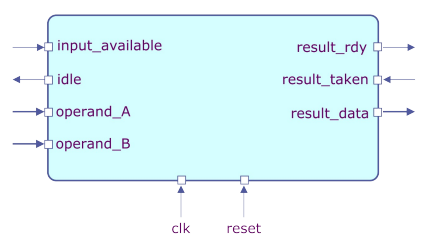
\includegraphics[width=15cm,angle=0]{imgs/diagram_block_top_level.png}
    \\\textbf{Fonte:} \cite{cse_taylor_michael}
    \label{fig:top_level}
\end{figure}

O diagrama de blocos na Figura \ref{fig:diagram_block} ilustra como os componentes principais
do sistema GCD se interconectam.

\begin{figure}[ht]
    \centering
    \caption{Diagrama de Blocos do Sistema GCD}
    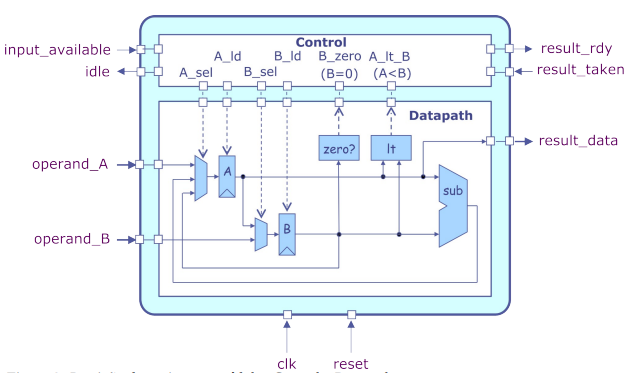
\includegraphics[width=17cm,angle=0]{imgs/diagram_block_control_datapath.png}
    \\\textbf{Fonte:} \cite{cse_taylor_michael}
    \label{fig:diagram_block}
\end{figure}

O Datapath inclui os registradores, multiplexadores e a unidade de subtração,
enquanto o Control FSM gerencia as operações com base nos sinais de controle.

\clearpage
\section{Desenvolvimento e Implementação}

Os materiais e métodos utilizados no desenvolvimento da pesquisa
incluem a descrição do algoritmo em C e
a modelagem dos módulos de controle e datapath em Verilog.
Além da simulação utilizando o ambiente Intel Quartus.

\subsection{Descrição do Algoritmo em C}

O código a seguir é uma implementação da função GCD (Greatest Common Divisor - Maior Divisor Comum).
Essa função calcula o maior divisor comum entre dois números inteiros.

A função GCD recebe dois parâmetros: inA e inB,
que representam os dois números inteiros para os quais
queremos calcular o maior divisor comum.

O código utiliza um algoritmo chamado "algoritmo de Euclides"
para calcular o maior divisor comum.
O algoritmo de Euclides é baseado na observação de que
o maior divisor comum entre dois números não muda
se o menor número for subtraído do maior número repetidamente
até que um dos números seja igual a zero.

O algoritmo para cálculo do GCD pode ser implementado de diversas maneiras.
Abaixo, apresentamos uma implementação em linguagem C:

\begin{verbatim}
int GCD(int inA, int inB) {
    int swap;
    int done = 0;
    int A = inA;
    int B = inB;
    while (!done) {
        if (A < B) {
            swap = A;
            A = B;
            B = swap;
        } else if (B != 0) {
            A = A - B;
        } else {
            done = 1;
        }
    }
    return A;
}
\end{verbatim}


Aqui está uma explicação passo a passo do funcionamento do código:
\begin{enumerate}
    \item O código declara algumas variáveis locais: \texttt{swap}, \texttt{done}, \texttt{A} e \texttt{B}. \texttt{swap} é usada para trocar os valores de \texttt{A} e \texttt{B} quando necessário. \texttt{done} é uma variável de controle que indica se o cálculo do maior divisor comum está concluído. \texttt{A} e \texttt{B} são inicializadas com os valores dos parâmetros \texttt{inA} e \texttt{inB}, respectivamente.
    \item O código entra em um loop \texttt{while} que continua até que a variável \texttt{done} seja igual a 1.
    \item O loop é usado para realizar as iterações necessárias para calcular o maior divisor comum.
    \item Dentro do loop, há uma estrutura \texttt{if-else} que verifica três condições:
    \begin{enumerate}
        \item Se \texttt{A} for menor que \texttt{B}, os valores de \texttt{A} e \texttt{B} são trocados usando a variável \texttt{swap}. Isso garante que \texttt{A} seja sempre o maior número.
        \item Se \texttt{B} for diferente de zero, \texttt{A} é atualizado para \texttt{A - B}. Isso realiza a subtração repetida até que um dos números seja igual a zero.
        \item Se nenhuma das condições anteriores for verdadeira, significa que o cálculo do maior divisor comum está concluído e a variável \texttt{done} é definida como 1 para sair do loop.
    \end{enumerate}
    \item Após o loop, o código retorna o valor de \texttt{A}, que representa o maior divisor comum entre os números \texttt{inA} e \texttt{inB}.
\end{enumerate}

Por exemplo, se chamarmos a função GCD(24, 36), o algoritmo de Euclides será aplicado da seguinte maneira:

\begin{enumerate}
    \item Na primeira iteração, \texttt{A} é atualizado para 36 e \texttt{B} é atualizado para 24.
    \item Na segunda iteração, \texttt{A} é atualizado para 12 e \texttt{B} é atualizado para 24.
    \item Na terceira iteração, \texttt{A} é atualizado para 12 e \texttt{B} é atualizado para 12.
    \item Na quarta iteração, \texttt{A} é atualizado para 0 e \texttt{B} é atualizado para 12.
    \item Como \texttt{B} é igual a zero, o cálculo do maior divisor comum está concluído e o valor retornado é 12.
\end{enumerate}

\subsection{Modelagem em Verilog}

A implementação do GCD em hardware envolve a
criação de módulos para o controle e o datapath.
O datapath lida com a movimentação e transformação dos dados,
enquanto o módulo de controle gerencia as operações de controle.

\subsubsection{Módulo Datapath}

O código a seguir é um exemplo de um módulo em Verilog
que implementa o datapath para um algoritmo de cálculo do
Máximo Divisor Comum (GCD - Greatest Common Divisor).

\begin{verbatim}
module GCDdatapath#( parameter W=16 )
(
    input clk,
    input [W-1:0] operand_A,
    input [W-1:0] operand_B,
    output [W-1:0] result_data,
    input A_ld,
    input B_ld,
    input [1:0] A_sel,
    input B_sel,
    output B_zero,
    output A_lt_B,
    output [W-1:0] A_chk, B_chk, sub_chk, A_mux_chk, B_mux_chk
);

    wire [W-1:0] A;
    wire [W-1:0] B;
    wire [W-1:0] sub_out;
    wire [W-1:0] A_mux_out;
    wire [W-1:0] B_mux_out;

    Mux3#(W) A_mux(
        .in0 (operand_A),
        .in1 (sub_out),
        .in2 (B),
        .sel (A_sel),
        .out (A_mux_out) 
    );

    register#(W) A_reg (
        .clk (clk),
        .d (A_mux_out),
        .en (A_ld),
        .q (A) 
    );

    Mux2#(W) B_mux (
        .in0 (A),
        .in1 (operand_B),
        .sel (B_sel),
        .out (B_mux_out) 
    );

    register#(W) B_reg (
        .clk (clk),
        .d (B_mux_out),
        .en (B_ld),
        .q (B) 
    );

    assign B_zero = (B==0);
    assign A_lt_B = (A < B);
    assign sub_out = A - B;
    assign result_data = A;
    // send checking signals only for debugging purposes
    assign A_chk = A;
    assign B_chk = B;
    assign sub_chk = sub_out;
    assign A_mux_chk = A_mux_out;
    assign B_mux_chk = B_mux_out;
endmodule
\end{verbatim}


A seguir, o funcionamento do código passo a passo:

O módulo GCDdatapath recebe alguns parâmetros,
sendo o principal deles W,
que define o tamanho dos operandos e do resultado em bits.

O módulo possui várias entradas e saídas, incluindo:

\begin{itemize}
    \item \texttt{clk}: um sinal de clock para sincronizar as operações.
    \item \texttt{operand\_A} e \texttt{operand\_B}: os operandos de entrada para o cálculo do GCD.
    \item \texttt{result\_data}: o resultado do cálculo do GCD.
    \item \texttt{A\_ld} e \texttt{B\_ld}: sinais de controle para carregar os operandos A e B.
    \item \texttt{A\_sel} e \texttt{B\_sel}: sinais de seleção para escolher entre os operandos A e B.
    \item \texttt{B\_zero}: um sinal indicando se o operando B é igual a zero.
    \item \texttt{A\_lt\_B}: um sinal indicando se o operando A é menor que o operando B.
    \item \texttt{A\_chk}, \texttt{B\_chk}, \texttt{sub\_chk}, \texttt{A\_mux\_chk} e \texttt{B\_mux\_chk}: sinais de depuração para verificar os valores internos do datapath.
\end{itemize}

O módulo possui várias fiações (wires) para conectar os componentes internos: \texttt{A}, \texttt{B}, \texttt{sub\_out}, \texttt{A\_mux\_out} e \texttt{B\_mux\_out}, que transportam os valores dos operandos e resultados intermediários.

O módulo utiliza vários componentes internos para realizar as operações do datapath:

\begin{itemize}
    \item \texttt{Mux3\#(W) A\_mux}: um multiplexador de 3 entradas que seleciona entre o operando A, o resultado da subtração e o operando B, com base no sinal de seleção \texttt{A\_sel}. O resultado é armazenado em \texttt{A\_mux\_out}.
    \item \texttt{register\#(W) A\_reg}: um registrador que armazena o valor de \texttt{A\_mux\_out} e o atualiza no sinal de clock \texttt{clk} quando o sinal de controle \texttt{A\_ld} está ativo. O valor atualizado é armazenado em \texttt{A}.
    \item \texttt{Mux2\#(W) B\_mux}: um multiplexador de 2 entradas que seleciona entre o valor atualizado de \texttt{A} e o operando \texttt{B}, com base no sinal de seleção \texttt{B\_sel}. O resultado é armazenado em \texttt{B\_mux\_out}.
    \item \texttt{register\#(W) B\_reg}: um registrador que armazena o valor de \texttt{B\_mux\_out} e o atualiza no sinal de clock \texttt{clk} quando o sinal de controle \texttt{B\_ld} está ativo. O valor atualizado é armazenado em \texttt{B}.
\end{itemize}

As atribuições \texttt{assign} são usadas para definir os valores das saídas do módulo:

\begin{itemize}
    \item \texttt{B\_zero} é atribuído como verdadeiro se o valor de \texttt{B} for igual a zero.
    \item \texttt{A\_lt\_B} é atribuído como verdadeiro se o valor de \texttt{A} for menor que o valor de \texttt{B}.
    \item \texttt{sub\_out} é atribuído como a diferença entre \texttt{A} e \texttt{B}.
    \item \texttt{result\_data} é atribuído como o valor de \texttt{A}.
    \item Os sinais de depuração \texttt{A\_chk}, \texttt{B\_chk}, \texttt{sub\_chk}, \texttt{A\_mux\_chk} e \texttt{B\_mux\_chk} são atribuídos aos respectivos valores internos do datapath.
\end{itemize}


O módulo GCDdatapath encapsula todas essas operações e fiações para formar um datapath completo para o cálculo do GCD.


\subsubsection{Módulo Controle}

O código abaixo é a implementação de um módulo de controle em Verilog, 
uma linguagem de descrição de hardware. 
Esse módulo de controle é chamado "GCDcontrol" e é usado para 
controlar o fluxo de um algoritmo de cálculo do maior divisor comum (GCD).

\begin{verbatim}
module GCDcontrol(
    input input_available,
    output reg idle,
    input clk, reset,
    output reg A_ld, B_sel, B_ld,
    output reg [1:0] A_sel,
    input B_zero, A_lt_B,
    output reg result_rdy,
    input result_taken,
    output [1:0] State
);

    // States naming
    localparam WAIT = 2'd0;
    localparam CALC = 2'd1;
    localparam DONE = 2'd2;

    // Constants naming for A_mux selector
    localparam A_SEL_IN = 2'b00;
    localparam A_SEL_SUB = 2'b01;
    localparam A_SEL_B = 2'b10;
    localparam A_SEL_X = 2'b11;
    // Constants naming for B_mux selector
    localparam B_SEL_A = 1'b0;
    localparam B_SEL_IN = 1'b1;
    localparam B_SEL_X = 1'bx;

    reg [1:0] CurrentState, NextState;

    always @(posedge clk or posedge reset)  
    begin 
        if (reset) 
            CurrentState <= WAIT;
        else 
            CurrentState <= NextState; 
    end 

    always @(CurrentState)
    begin
        // default is to stay in the same state
        NextState <= CurrentState;
        case ( CurrentState )
            WAIT :
                if ( input_available )
                    NextState <= CALC;
            CALC :
                if ( B_zero )
                    NextState <= DONE;
            DONE :
                if ( result_taken )
                    NextState <= WAIT;
        endcase
    end 

    always @( * )
    begin
        // Default control signals
        A_sel <= A_SEL_X;
        A_ld <= 1'b0;
        B_sel <= B_SEL_X;
        B_ld <= 1'b0;
        idle <= 1'b0; 
        result_rdy = 1'b0;

        case ( CurrentState )
            WAIT :
                begin
                    idle <= 1'b1; 
                    if(input_available)begin
                        A_sel <= A_SEL_IN;
                        B_sel <= B_SEL_IN;
                        A_ld <= 1'b1;   
                        B_ld <= 1'b1;
                    end
                end
            CALC :
                if ( A_lt_B )begin
                    A_sel <= A_SEL_B;
                    B_sel <= B_SEL_A;
                    A_ld <= 1'b1;
                    B_ld <= 1'b1;
                end
                else if ( !B_zero )begin
                    A_sel <= A_SEL_SUB;
                    A_ld <= 1'b1;
                end
            DONE : 
                result_rdy <= 1'b1;
        endcase
    end

    assign State = CurrentState;
endmodule
\end{verbatim}


Analisando o código passo a passo:

\begin{enumerate}
    \item O módulo "GCDcontrol" possui várias entradas e saídas, que são definidas na lista de portas do módulo.
    As entradas incluem \texttt{input\_available}, \texttt{clk}, \texttt{reset}, \texttt{B\_zero} e \texttt{A\_lt\_B}, enquanto as saídas incluem \texttt{idle}, \texttt{A\_ld}, \texttt{B\_sel}, \texttt{B\_ld}, \texttt{A\_sel}, \texttt{result\_rdy} e \texttt{State}.
    \item O módulo também define alguns parâmetros locais, como os nomes dos estados e as constantes para os seletores de multiplexadores.
    \item O módulo possui duas variáveis de estado, \texttt{CurrentState} e \texttt{NextState}, que são atualizadas em um bloco \texttt{always} sensível à borda de subida do sinal de clock ou de reset.
    \item Em seguida, há um bloco \texttt{always} sensível ao valor de \texttt{CurrentState}, que determina o próximo estado com base no estado atual. O próximo estado é atribuído à variável \texttt{NextState} usando uma estrutura \texttt{case} que verifica o valor de \texttt{CurrentState} e toma decisões com base nesse valor.
    \item O próximo bloco \texttt{always} é sensível a todas as mudanças de sinal e é usado para definir os sinais de controle com base no estado atual. Ele define os valores dos sinais \texttt{A\_sel}, \texttt{A\_ld}, \texttt{B\_sel}, \texttt{B\_ld}, \texttt{idle} e \texttt{result\_rdy} com base no valor de \texttt{CurrentState}. Novamente, uma estrutura \texttt{case} é usada para tomar decisões com base no estado atual.
    \item Por fim, o sinal \texttt{State} é atribuído ao valor de \texttt{CurrentState} usando a declaração \texttt{assign}.
\end{enumerate}

Em resumo, esse módulo de controle implementa a lógica para controlar o fluxo de um algoritmo de cálculo do maior divisor comum. Ele define os estados do algoritmo e os sinais de controle necessários para executar as operações corretas em cada estado.

\section{Máquina de Estados Finitos (FSM)}
% Nesta seção, discuta a FSM utilizada para controlar o Datapath.
A máquina de estados finitos (FSM) é uma abordagem essencial
para controlar o fluxo de operações em um sistema digital,
especialmente na implementação de algoritmos como o cálculo
do Greatest Common Divisor (GCD). A FSM divide o processo
de cálculo em diferentes estados, cada um representando uma
etapa específica na operação, e controla a transição entre
esses estados com base nas condições de entrada e saídas
esperadas. A figura abaixo (FIGURA 1) mostra a FSM utilizada para controlar
o datapath do GCD.

\begin{figure}[ht]
    \centering
    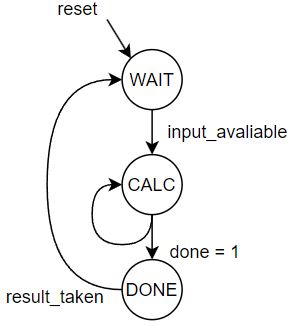
\includegraphics[width=7cm,angle=0]{imgs/state_machine_GCD.png}
    \caption{Máquina de Estados Finitos para o GCD}
    \label{fig:fsm}
\end{figure}

\subsection{Descrição dos Estados}
% Descrever os diferentes estados da FSM, explicando o que ocorre em cada estado e como as transições entre estados são gerenciadas. Pode incluir um diagrama de estados para visualização.
A FSM apresentada na figura contém três estados principais:
\textit{WAIT}, \textit{CALC}, e \textit{DONE}. Cada estado desempenha um papel crucial
no ciclo de vida do cálculo do \textit{GCD}:
\subsubsection{Estado \textit{WAIT} (Aguardando novos operandos)}
Este é o estado inicial da FSM, onde o sistema está inativo e
aguardando a disponibilidade de novos operandos para iniciar o
cálculo. Neste estado, o sistema verifica a sinalização de
disponibilidade de entrada (\textbf{input\_available}). Quando
a sinalização \textbf{input\_available} é ativada, indicando que
os operandos estão prontos para serem processados, a FSM
transita para o estado \textit{CALC}.

\subsubsection{Estado CALC (Calculando o GCD)}
Neste estado, o algoritmo de Euclides é executado, onde
os valores dos operandos são trocados e subtraídos
repetidamente até que o menor dos dois operandos seja zero.
Este processo continua até que a condição de término seja
atingida (\textit{done} = 1), o que indica que o GCD foi encontrado.
A FSM permanece neste estado enquanto a condição \textit{done} = 1
não é satisfeita. Quando a condição \textit{done} = 1 é atingida,
o sistema transita para o estado \textit{DONE}.

\subsubsection{Estado DONE (Esperando o consumidor receber o resultado)}
No estado \textit{DONE}, o sistema aguarda que o consumidor ou a
unidade de processamento a jusante receba o resultado do
cálculo do \textit{GCD}. Durante este estado, o sistema está
essencialmente "em espera", até que o sinal \textbf{result\_taken}
seja ativado.Após o sinal \textbf{result\_taken} ser ativado,
indicando que o resultado foi processado ou consumido,
a \textit{FSM} retorna ao estado \textit{WAIT} para reiniciar o ciclo
com novos operandos.


\subsection{Implementação da FSM}
% Discutir como a FSM foi implementada em Verilog, incluindo os desafios encontrados durante o desenvolvimento e como foram superados. Explicar a lógica de transição e os sinais de controle envolvidos.

A FSM foi implementada em Verilog, utilizando registradores
para armazenar o estado atual e o próximo estado, e lógica
combinacional. É possivel separar a implementação da FSM em
três partes principais: a definição dos estados e sinais de
controle, a lógica de transição de estados, e a lógica de
controle de sinais.

\subsubsection{Definição dos Estados e Sinais de Controle}
O FSM tem três estados principais definidos como constantes locais (\textit{localparam}):

\begin{verbatim}
        localparam WAIT = 2'd0;
        localparam CALC = 2'd1;
        localparam DONE = 2'd2;
\end{verbatim}

Os sinais de controle da FSM são definidos como registradores de saída (\textit{reg}):
\begin{verbatim}
        output reg idle,
        output reg A_ld, B_sel, B_ld,
        output reg [1:0] A_sel,
        output [1:0] State
        output reg result_rdy,
\end{verbatim}

Tambem são definidos constantes para os seletores dos multiplexadores A e B:
\begin{verbatim}
        // constants naming for A_mux selector
        localparam A_SEL_IN = 2'b00;
        localparam A_SEL_SUB = 2'b01;
        localparam A_SEL_B = 2'b10;
        localparam A_SEL_X = 2'b11;

        // constants naming for B_mux selector
        localparam B_SEL_A = 1'b0;
        localparam B_SEL_IN = 1'b1;
        localparam B_SEL_X = 1'bx;
\end{verbatim}

e os estados da FSM são definidos como registradores de 2 bits:
\begin{verbatim}
        reg [1:0] CurrentState, NextState;
\end{verbatim}

\subsubsection{Lógica de Controle de Sinais}
A FSM é implementada em duas partes principais: a lógica de transição de estados e a lógica de controle de sinais. A lógica de transição de estados é baseada em um bloco \textit{always} que
atualiza o estado atual (\textit{CurrentState}) com base no próximo estado (\textit{NextState}):
\begin{verbatim}
    always @(posedge clk or posedge reset)  
    begin 
        // reset the FSM to the initial state when reset signal is active
        if (reset) 
            CurrentState <= WAIT;
        else 
            CurrentState <= NextState; 
    end 

    always @(CurrentState)
    begin
        // default is to stay in the same state
        NextState <= CurrentState;
        case ( CurrentState )
            WAIT :
                if ( input_available )
                    NextState <= CALC;
            CALC :
                if ( B_zero )
                    NextState <= DONE;
            DONE :
                if ( result_taken )
                    NextState <= WAIT;
        endcase
    end
\end{verbatim}

\subsubsection{Controle de Sinais}

A lógica de controle de sinais é implementada em um bloco \textit{always} que define os sinais de controle com base no estado atual da FSM:

\begin{verbatim}
    always @( * )
    begin
        // Default control signals
        A_sel <= A_SEL_X;
        A_ld <= 1'b0;
        B_sel <= B_SEL_X;
        B_ld <= 1'b0;
        idle <= 1'b0; 
        result_rdy = 1'b0;

        case ( CurrentState )
            WAIT :
                begin
                    idle <= 1'b1; 
                    if(input_available)begin
                        A_sel <= A_SEL_IN;
                        B_sel <= B_SEL_IN;
                        A_ld <= 1'b1;   
                        B_ld <= 1'b1;
                    end
                end
            CALC :
                if ( A_lt_B )begin
                    A_sel <= A_SEL_B;
                    B_sel <= B_SEL_A;
                    A_ld <= 1'b1;
                    B_ld <= 1'b1;
                end
                else if ( !B_zero )begin
                    A_sel <= A_SEL_SUB;
                    A_ld <= 1'b1;
                end
            DONE : 
                result_rdy <= 1'b1;
        endcase
    end
\end{verbatim}

\section{Simulações e Verificação}

% Descrever o ambiente de simulação utilizado, como o Intel QuestaSim. Explicar como os testes foram configurados e quais aspectos do sistema foram verificados.
A simulação do módulo de controle GCD foi realizada
utilizando o Software Quartus, um ambiente de
desenvolvimento amplamente utilizado para projetos
de FPGA. O objetivo dessa simulação é validar a
implementação da Máquina de Estados Finitos (FSM)
que controla o processo de cálculo do Greatest
Common Divisor (GCD) e verificar se os sinais de
controle e estado estão funcionando conforme o
esperado.

\subsection{Ambiente de Simulação}
O ambiente de simulação foi configurado no Quartus para testar o módulo \texttt{GCDcontrol}, responsável por coordenar as operações necessárias para calcular o GCD. A simulação foi conduzida com os seguintes sinais principais:
\begin{itemize}
    \item \textbf{clk}: Sinal de clock que sincroniza as operações do módulo.
    \item \textbf{reset}: Sinal de reset utilizado para reinicializar a FSM ao estado inicial (\texttt{WAIT}).
    \item \textbf{input\_available}: Sinal de controle que indica a disponibilidade de novos operandos de entrada.
    \item \textbf{B\_zero}: Sinal de feedback do datapath indicando que o valor de B é zero, o que significa que o cálculo do GCD foi concluído.
    \item \textbf{result\_taken}: Sinal de controle indicando que o resultado foi processado ou consumido.
    \item \textbf{A\_lt\_B}: Sinal que indica se o valor de A é menor que B, usado para determinar a troca de valores.
    \item \textbf{A\_sel, B\_sel, A\_ld, B\_ld}: Sinais de controle para a seleção e carregamento dos registradores no datapath.
    \item \textbf{idle, result\_rdy, State}: Sinais de saída do módulo de controle indicando o estado atual da FSM, se o sistema está inativo (\texttt{idle}), e se o resultado está pronto para ser processado (\texttt{result\_rdy}).
\end{itemize}

A simulação foi conduzida utilizando o Software Quartus, que é amplamente utilizado para o desenvolvimento e verificação de projetos de FPGA. Os sinais mencionados foram monitorados ao longo do tempo para verificar se o módulo \texttt{GCDcontrol} opera conforme o esperado, garantindo a correta transição de estados e o comportamento desejado da FSM.
\subsection{Resultados da Simulação}
% Apresentar os resultados obtidos durante a simulação. Incluir gráficos ou capturas de tela que mostrem a operação do GCD. Discutir se os resultados atenderam às expectativas e os objetivos do projeto.

A captura de tela fornecida (Figura \ref{simulacao_gcd}) mostra a forma de onda gerada durante a simulação no Quartus.

\begin{figure}[ht]
    \centering
    \caption{Simulação do Módulo de Controle GCD}
    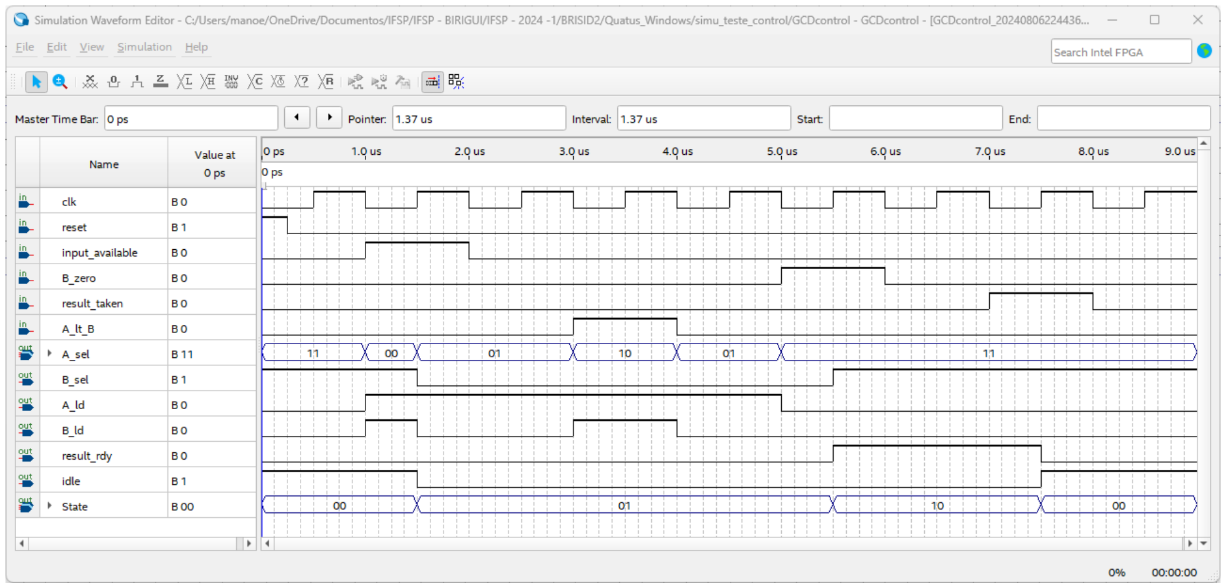
\includegraphics[width=15cm,angle=0]{imgs/simulacao_gcd_quartus.png}
    \\\textbf{Fonte:} Elaborado pelos autores
    \label{simulacao_gcd}
\end{figure}

A análise dos resultados da simulação pode ser dividida em várias fases, conforme mostrado na forma de onda simulada. Cada fase representa um conjunto de operações e transições de estado na FSM:

\subsubsection{Inicialização e Reset (0.0 µs - 1.0 µs)}

No início da simulação, o sinal \texttt{reset} é ativado (\texttt{1}), o que força a FSM a reiniciar no estado \texttt{WAIT} (indicando por \texttt{State = 00}). Esse estado inicial é crucial, pois garante que o sistema comece em uma condição conhecida e estável. Durante esse período, o sinal \texttt{idle} também está ativado, indicando que o sistema está em um estado inativo, aguardando a disponibilidade de novos operandos para iniciar o cálculo.

\subsubsection{Disponibilidade de Entradas e Transição para CALC (1.0 µs - 2.0 µs)}

Após a fase de reset, o sinal \texttt{input\_available} é ativado (\texttt{1}), sinalizando que os operandos de entrada estão prontos para serem processados. Como resposta, a FSM transita do estado \texttt{WAIT} para o estado \texttt{CALC} (\texttt{State = 01}). Nesta fase, os sinais de controle \texttt{A\_sel} e \texttt{B\_sel} são configurados para selecionar os operandos corretos, e os sinais \texttt{A\_ld} e \texttt{B\_ld} são ativados (\texttt{1}), permitindo que os valores dos operandos sejam carregados nos registradores correspondentes no datapath. Esta transição é essencial para iniciar o processo de cálculo do GCD.

\subsubsection{Cálculo e Subtrações (2.0 µs - 6.0 µs)}

Durante o estado \texttt{CALC}, a FSM realiza as operações necessárias para o cálculo do GCD. Neste ponto, a FSM continua no estado \texttt{CALC}, alternando entre subtrações e comparações, conforme determinado pelo sinal \texttt{A\_lt\_B}, que indica se o valor de \texttt{A} é menor que \texttt{B}. As operações de subtração continuam até que o sinal \texttt{B\_zero} seja ativado, indicando que o valor de \texttt{B} chegou a zero, o que significa que o GCD foi encontrado. Durante essa fase, a FSM coordena as operações de subtração e troca de valores no datapath, utilizando os sinais \texttt{A\_sel} e \texttt{B\_sel} para garantir que as operações sejam realizadas corretamente.

\subsubsection{Conclusão do Cálculo e Transição para DONE (6.0 µs - 7.0 µs)}

Quando o sinal \texttt{B\_zero} é ativado, a FSM reconhece que o cálculo do GCD foi concluído. Nesse momento, a FSM transita do estado \texttt{CALC} para o estado \texttt{DONE} (\texttt{State = 10}). No estado \texttt{DONE}, o sinal \texttt{result\_rdy} é ativado, indicando que o resultado do GCD está pronto para ser consumido ou processado pela próxima etapa do sistema. Esta transição é crucial para finalizar o ciclo de cálculo e preparar o sistema para a próxima operação.

\subsubsection{Consumo do Resultado e Retorno ao Estado WAIT (7.0 µs - 9.0 µs)}

Após o cálculo ser concluído, o sinal \texttt{result\_taken} é ativado, indicando que o resultado foi processado ou retirado pelo sistema consumidor. Em resposta, a FSM retorna ao estado \texttt{WAIT}, reiniciando o ciclo de operação. O sistema agora está pronto para receber novos operandos e repetir o processo de cálculo do GCD. Essa fase final assegura que a FSM está pronta para iniciar novamente, mantendo a continuidade do fluxo de operações.

\section{Otimizações e Melhorias Futuras}

Mesmo se tratando de um algoritmo relativamente simples, o design do GCD em hardware pode ser otimizado e expandido para atender a requisitos mais exigentes. Nesta seção, discutiremos possíveis melhorias no design, como a implementação de pipelining no datapath e a expansão do sistema para suportar operações mais complexas.




\subsection{Otimização do Datapath}
% Sugerir melhorias no Datapath, como a implementação de pipelining para aumentar a eficiência. Discutir possíveis modificações que poderiam ser feitas para melhorar o desempenho geral do sistema.
Uma possível otimização é a implementação de pipelining no datapath. Isso permitiria que várias operações de subtração e troca fossem executadas em paralelo, aumentando a eficiência do sistema. Além disso, o uso de registradores adicionais poderia reduzir o número de operações de leitura e escrita na memória, melhorando ainda mais o desempenho.


\subsubsection{Implemetação do Pipelining}
O pipelining é uma técnica fundamental para aumentar a eficiência e o desempenho de sistemas de processamento. Ao aplicar pipelining no datapath do algoritmo GCD, podemos dividir o processo de cálculo em estágios distintos que podem ser executados em paralelo, reduzindo o tempo total necessário para a execução e aumentando o throughput \cite{Hennessy2017}.

\begin{enumerate}
\item \textbf{Divisão do Algoritmo GCD em Estágios}



Para o algoritmo GCD, que geralmente é implementado usando o Algoritmo de Euclides, podemos dividir o processamento em vários estágios:

\begin{itemize}
    \item \textbf{Estágio 1:} Cálculo do Resto - Calcula o resto da divisão entre dois números.
    \item \textbf{Estágio 2:} Atualização dos Valores - Atualiza os valores dos números com base no resto calculado.
    \item \textbf{Estágio 3:} Verificação da Condição de Parada - Verifica se o resto é zero, o que indica que o cálculo está concluído \cite{Knuth1997}.
\end{itemize}

\item \textbf{Implementação do Pipelining}

A implementação do pipelining para o GCD pode ser feita da seguinte maneira:

\begin{itemize}
    \item \textbf{Pipeline de Estágios}: Cada estágio do pipeline pode ser otimizado para realizar sua tarefa específica simultaneamente com outros estágios. Por exemplo, enquanto um estágio calcula o resto, outro pode estar atualizando os valores ou verificando a condição de parada.
    \item \textbf{Buffer de Pipeline}: Adicionar buffers entre os estágios para armazenar dados temporários e permitir que o processamento continue sem interrupções.
    \item \textbf{Controle de Fluxo}: Implementar mecanismos de controle para gerenciar a sincronização entre os estágios e garantir que cada estágio receba os dados no momento certo \cite{Patterson2013}.
\end{itemize}

\end {enumerate}

\subsubsection{Benefícios do Pipelining}

\begin{enumerate}
    \item \textbf{Redução do Tempo de Execução} Ao dividir o trabalho entre vários estágios e processar diferentes partes do algoritmo simultaneamente, o tempo total para concluir a operação de GCD é reduzido.
    \item \textbf{Aumento do Throughput:} A capacidade de processar múltiplos cálculos de GCD em paralelo pode aumentar o throughput geral do sistema \cite{Harris2010}.
    \item \textbf{Paralelismo de dados:}
          \begin{itemize}
              \item \textbf{Execução Paralela:} Implementar execução paralela para processar múltiplos pares de números simultaneamente. Isso pode ser feito usando múltiplos pipelines ou unidades de processamento.
          \end{itemize}
    \item \textbf{Otimização de Hardware:}
          \begin{itemize}
              \item \textbf{Uso de Recursos Específicos:} Utilizar unidades de hardware específicas para operações matemáticas, como divisores de alto desempenho, para acelerar o cálculo do resto.
              \item \textbf{Redução de Latência:} Minimizar a latência entre as operações utilizando técnicas de otimização de circuito.
              \item \textbf{Eficiência Energética:} Implementar técnicas para reduzir o consumo de energia, como a otimização do design do circuito e o uso eficiente dos recursos de hardware.
          \end{itemize}
    \item \textbf{Algoritmos Alternativos:}
          \begin{itemize}
              \item \textbf{Exploração de Algoritmos:} Explorar algoritmos alternativos para o cálculo do GCD que possam oferecer melhorias em termos de eficiência e velocidade \cite{Skiena2008}.
          \end{itemize}
\end{enumerate}

% Redução do Tempo de Execução: Ao dividir o trabalho entre vários estágios e processar diferentes partes do algoritmo simultaneamente, o tempo total para concluir a operação de GCD é reduzido.
% Aumento do Throughput: A capacidade de processar múltiplos cálculos de GCD em paralelo pode aumentar o throughput geral do sistema \cite{Harris2010}.
% Possíveis Modificações para Melhorar o Desempenho
% Além do pipelining, outras modificações podem ser feitas para melhorar o desempenho geral do sistema:

% 1. Paralelismo de Dados

% Execução Paralela: Implementar execução paralela para processar múltiplos pares de números simultaneamente. Isso pode ser feito usando múltiplos pipelines ou unidades de processamento.
% 2. Otimização de Hardware

% Uso de Recursos Específicos: Utilizar unidades de hardware específicas para operações matemáticas, como divisores de alto desempenho, para acelerar o cálculo do resto.
% Redução de Latência: Minimizar a latência entre as operações utilizando técnicas de otimização de circuito.
% 3. Eficiência Energética

% Otimização de Consumo de Energia: Implementar técnicas para reduzir o consumo de energia, como a otimização do design do circuito e o uso eficiente dos recursos de hardware.
% 4. Algoritmos Alternativos

% Exploração de Algoritmos: Explorar algoritmos alternativos para o cálculo do GCD que possam oferecer melhorias em termos de eficiência e velocidade \cite{Bressoud2011}.
\paragraph{Conclusão :}
A aplicação de pipelining e outras técnicas de otimização pode significativamente melhorar a eficiência e o desempenho do datapath para o algoritmo GCD. Ao dividir o trabalho em estágios e implementar estratégias para reduzir latência e aumentar o throughput, podemos alcançar um sistema mais rápido e eficiente.


\subsection{Expansão do Design para Sistemas Maiores}
% Discutir como o design do GCD poderia ser expandido para se integrar com sistemas maiores ou suportar operações mais complexas. Propor ideias para a adaptação do módulo para novas aplicações.

Outra melhoria futura seria a expansão do design para suportar sistemas maiores ou operações mais complexas. Por exemplo, o módulo GCD poderia ser integrado a um processador ou coprocessador específico para criptografia. Isso exigiria a adaptação do módulo para se comunicar com outros componentes do sistema e lidar com algoritmos mais avançados.




\section{Discussão sobre Integração com Sistemas Maiores e Otimização do Datapath}
% Explorar como o módulo GCD poderia ser integrado em sistemas mais complexos, como processadores ou coprocessadores específicos para criptografia. Discutir os desafios de integração e as vantagens dessa abordagem.

É importante ressaltar que essas otimizações e melhorias futuras podem trazer desafios adicionais, como a complexidade do design e a necessidade de recursos adicionais. Portanto, é necessário realizar uma análise cuidadosa dos requisitos e restrições do sistema antes de implementar essas melhorias.


Em resumo, as otimizações e melhorias futuras no design do algoritmo GCD em hardware são uma área de interesse contínua para estudantes de Engenharia de Computação. Com a combinação certa de conhecimento teórico e prático, é possível criar soluções eficientes e inovadoras que atendam às demandas cada vez maiores da computação moderna.


\section{Conclusões}

Neste artigo, apresentamos a implementação do algoritmo GCD em hardware, detalhando a modelagem dos módulos de controle e datapath em Verilog. A simulação mostrou que a abordagem utilizada é eficiente e atende aos requisitos do projeto. Em conclusão, a implementação do Algoritmo de Euclides para o cálculo do GCD exemplifica a intersecção eficaz entre teoria matemática e aplicações práticas em hardware digital. Através do uso de registradores, multiplexadores e unidades aritméticas, o algoritmo é traduzido em circuitos de controle e datapath que executam operações iterativas de forma eficiente.
Esse processo é fundamental para diversos contextos, incluindo criptografia, compressão de dados e controle de hardware, demonstrando a versatilidade e a importância do GCD em sistemas computacionais modernos. A clareza na separação entre os módulos de controle e datapath não só facilita a implementação e manutenção do sistema, mas também otimiza seu desempenho, especialmente em aplicações que demandam alta velocidade e economia de recursos. As melhorias propostas, como a implementação do pipelining e a otimização do datapath, revelam o potencial para aumentar ainda mais a eficiência do cálculo do GDC. O pipelining, ao permitir que várias operações ocorram simultaneamente, pode reduzir significativamente o tempo de execução e aumentar a capacidade de processamento do sistema.
Essas melhorias, juntamente com a possibilidade de expandir o design para suportar sistemas maiores e operações mais complexas, apontam para um caminho promissor na evolução do design de hardware digital. 

O desafio, entretanto, reside na necessidade de equilibrar a complexidade do design com os recursos disponíveis, garantindo que as soluções sejam não apenas eficientes, mas também praticas e sustentáveis. Com uma análise cuidadosa das restrições e demandas do sistema, é possível criar designs inovadores que atendam às crescentes necessidades da computação moderna, proporcionando um desempenho superior e uma maior eficiência energética. Em suma, as otimizações no algoritmo GCD e sua integração em sistemas maiores representam uma área de estudo contínua e vital para o avanço da engenharia da computação.

%Referências Bibliográficas
\bibliography{bibliografia.bib}
%\printbibliography[title={REFERÊNCIAS}]
%\printbibliography{bibliografia}

\end{document}
